 \documentclass[]{report}
%\documentclass[10pt,a4paper,headinclude=true,twoside]{report}
\usepackage[latin1]{inputenc}
\usepackage[a4paper]{geometry}
\usepackage{a4wide}
\usepackage{amsmath}
\usepackage{amsfonts}
\usepackage{amssymb}
\usepackage{graphicx}
\usepackage{hyperref}
\usepackage{pdflscape} % dlia landscape orientation 
\hypersetup{colorlinks,citecolor=black,filecolor=black,linkcolor=black,urlcolor=black}
\usepackage{float}
\usepackage{setspace}
\usepackage{titlesec}


\begin{document}
%\onehalfspacing
\title{CS31310: Process for project}
\author{Edgar Ivanov\\ edi@aber.ac.uk \\ Department of Computer Science, Aberystwyth University}
\date{\today}
\maketitle
\section*{Project outline}
My final year project will have both hardware and software parts. The aim of the project is to build additional unit which will ensure that camera mounted on the rover is always in stable position. Currently there is a Pan-and-Tilt Unit (PTU) which controls the camera and ensures that it is in a stable position. It uses gyroscopes to acquire current position in the space and based on that adjusts position of the camera. However gyroscopes are not perfect and tend to drift over the time, as well as provide wrong data at the different temperature. 

I will be building additional unit which will acquire current position using the more accurate accelerometer and then will provide PTU with the calibration data.

\section*{Process}
At this point it is difficult for me to choose the right development methodology for my project. There are a few of them and I have very limited experience of using any of them. Since I didn't go in too much details of my project yet, it will be a bit of guess work to try and find suitable methodology.

Essentially my customer will be my project supervisory, because I am building system for him and he has deep interest in this project being completed. There will be no big team of developers working on the project, just me with some help from my supervisor. The final goal of the project is clear and doesn't seem to be difficult to achieve, so it should be a matter of requirement analysis, design and implementation.

On the other hand, I have a very limited knowledge of C programming language and experience of working with proposed hardware, so for me it will be an exploratory work as well, to find out how to fit all the parts together and make them work. I may not be able to predict all the pitfalls on the course of the project and as such may need to revise and alter my plan. Having said that I need a flexible methodology, which allows for changes in requirements and design to be made during the development. 

The first thought was to adopt XP with some changes. It was attractive since it didn't require BDUF, documentation, requirements analysis and I could start coding straight away. Problem here would be with pair programming which I believe (after reading why XP is like a ring of poisonous snakes) is compulsory for XP, if there is no design, it is essential for somebody to sit next to you and double check all you do to catch design errors and this would not be possible on single person project. On-site customer is my next concern, I doubt my supervisor will be able to devote more than a few hours a week for this project, so I can't even speak about the customer being part of the development team, who is essential to make sure that final system meets customer expectations.

I also thought of waterfall model since I like to have some plan which I can follow, but as I said before I would need to make changes during the project and waterfall wouldn't be suitable. Spiral model was also considered, but after the deeper reading I found that it may not be suitable for the smaller projects.

After more research carried out in this field I decided to try and adapt evolutionary prototyping model. Prototype system will be built at the beginning and then during the course of the project I will be improving it according to the supervisors feedback, so that at the end it evolves in to the complete system. I might use throw-away prototype at the beginning to better understand the system requirements and then switch to the evolutionary prototyping, then it would becomes mix of the two life-cycle methodologies.

\begin{figure}[H]
\centering
\centerline{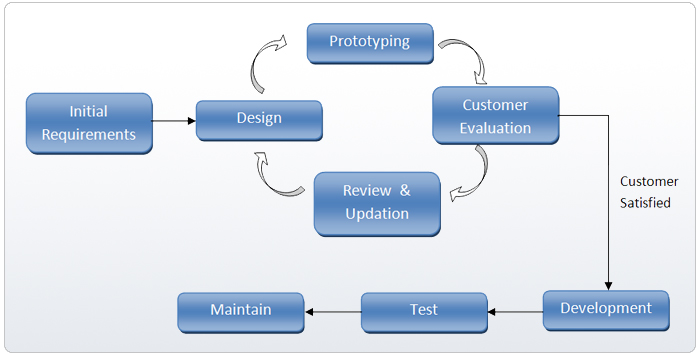
\includegraphics[scale=0.55]{./prototype_methodology}}
\caption{Prototyping model }
\label{fig:i-s-hierarchy-tree-march-2012}
\end{figure}


 
 references
 About poisonousness snakes
 bookmarked article
 
\end{document}